The goal of this chapter is to practice what was learnt previously. It discusses some examples of memory transfers among the host and \glspl{eCore} as well as the implementation of the linpack benchmark. Examples will provide some pieces of code and schemes to help understanding the processes explained.

\section[Example 1]{Example: Transfer between \gls{eCore} and Host}

Example available on \href{https://github.com/nkcr/parallella-computing/blob/master/simple-epiphany/}{GitHub}\cite{githubproject}: \textit{simple-epiphany/hello-from-epiphany}.

Figure \ref{fig epiphanyhost} is a summary of the operations we are going to do so as to transfer data between the \gls{epiphany} and the host part. We are going to:

\begin{enumerate}
  \item set a shared buffer from the host
  \item set a pointer to the shared buffer from the \gls{epiphany}, then write to it
  \item from the host, read data written from the epiphany to the shared buffer
\end{enumerate}

\begin{figure}[h!]
\centering
\includegraphics[width=0.7\textwidth]{examples/epiphanyhost.pdf}
\caption{Simplistic scheme of transferring data from epiphany to host}
\label{fig epiphanyhost}
\end{figure}

Setting a shared buffer from the host is achieved with \code{e\_alloc}. This method takes a variable's reference of type \code{e\_mem\_t} (representing the shared buffer) and allocs memory space on it. The following code declares our shared buffer then allocs a certain space.

\begin{lstlisting}
e_mem_t emem; // shared memory buffer
e_alloc(&emem, BUFOFFSET, sizeof(unsigned)*ncores);
\end{lstlisting}

As we will see in the other examples, \code{e\_alloc} allocates memory from address \code{0x8e00'0000}. Our linker description file (\gls{LDF}) tells us that shared memory is allocated from \code{0x8f00'0000}, thus we need an offset of \code{0x0100'0000} to start writing at the right address (\code{0x8e00'0000} + \code{0x8100'0000} =\\ \code{0x8f00'0000}).

To be able to write to this shared buffer from the \gls{eCore}, we need to set a pointer to the right address. In our case it will be \code{0x8f00'0000}. The following code, run by each \glspl{eCore}, sets a pointer beginning from \code{08f00'0000} plus an offset depending of each \gls{eCore}'s number. Then we write something to the buffer's address. Those data will be available from the host part. By doing so, we directly write to the memory shared buffer we set in the host part.

\begin{lstlisting}
volatile unsigned *result; // Pointer to the shared buffer
result  = (volatile unsigned *) (0x8f000000 
                                 + sizeof(unsigned)*num);
*result = num;
\end{lstlisting}

On the host, to finally read what \glspl{eCore} put, we use \code{e\_read} to copy the buffer data to a local variable. The following code places the data from our shared buffer to a local array and then prints the result.

\begin{lstlisting}
int result[ncores];
e_read(&emem, 0, 0, 0x0, result, ncores * sizeof(int));
for(i = 0; i < ncores; i++)
  printf("Result from core %02i is 0x%04x\n",i, result[i]);
\end{lstlisting}

\section[Example 2]{Example: Transfer between \gls{eCore} and \gls{eCore}}

Examples available on \href{https://github.com/nkcr/parallella-computing/blob/master/simple-epiphany/hello-from-neighbor-ecore/emain.c}{GitHub}\cite{githubproject}: \textit{simple-epiphany/hello-from-neighbor-ecore}.

In figure \ref{fig eCore to eCore}, we see that communicating from an \gls{eCore} to another will be achieved by using \glspl{eCore}' local memory. The \gls{SDK} gives us methods to manipulate data between each \glspl{eCore}. We are going to:

\begin{enumerate}
  \item from one \gls{eCore}, get the coordinates of it's neighbor
  \item given the coordinates, writing to the \gls{eCore}'s neighbor local memory
  \item from the neighbor \gls{eCore}, read local memory so as to get the data
\end{enumerate}


\begin{figure}[h!]
\centering
\includegraphics[width=0.7\textwidth]{examples/eCore_to_eCore.pdf}
\caption{Simplistic scheme of transferring data from an \gls{eCore} to another \gls{eCore}}
\label{fig eCore to eCore}
\end{figure}

Reading and writing from an \gls{eCore} to another one is achieved with \code{e\_read} and \code{e\_write}. Those methods take as parameter the row\_id and the col\_id of the \gls{eCore} we want to read/write. The \gls{SDK} gives us a method to get the coordinates of an \gls{eCore}'s neighbor. In the following code, written for an \gls{eCore}, we retrieve the coordinates of the neighbor and then read a char at its locale memory.

\begin{lstlisting}
  unsigned neighbor_row, neighbor_col;
  e_neighbor_id(E_NEXT_CORE, E_GROUP_WRAP, 
                &neighbor_row, &neighbor_col);
  e_read(&e_group_config,&neighbor_status,
         neighbor_row,neighbor_col,(char*)0x4000,1);
\end{lstlisting}

We note that we gave \code{0x4000} as the offset memory. That value corresponds to the relative offset memory of the local \gls{eCore}'s memory. As seen previously in this document, each \gls{eCore} has 4 banks of memory, starting from \code{0x0000} to \code{0x7fff}. Giving an offset of \code{0x4000} will read the data in the second bank of memory (see table \ref{table:eCore}).

From the target \gls{eCore}, to read the value set from the other \gls{eCore}, we must set a variable at the correct address. To make it easier, we declared a char array and specified its location to be on the second bank (hence starting at the address \code{0x4000}). We then used that array to manipulate the data. The following code shows us how we declared the array and how we read the data from the target \gls{eCore}:

\begin{lstlisting}
	char swap[8] SECTION(".text_bank2");
	swap[0] = core_num; // that data will be at 0x4000
	swap[1] = ...; // that data will be at 0x4001
\end{lstlisting}

The section used in our code (text\_bank2) is defined in the \gls{LDF}.

\subsection{Transfers times using different methods}

We used \code{e\_read} and \code{e\_write} to communicate between \glspl{eCore}. But there is two other options. In the following example, we will set each eCore to read it's neighbor memory and measure the time spent for each options. The three options are:
\begin{itemize}
  \item Using the function \code{e\_read} provided by the \gls{SDK} (as seen previously)
  \item Directly writing using the global address
  \item Using \gls{DMA}
\end{itemize}

According to the SDK reference, the function \code{e\_read} copy bytes of data from a remote source to a destination source \cite{epiphanySDK}. In our case, the destination is given by the coordinates of the \gls{eCore}. Our test uses the timer to count the number of clocks while we repeatedly perform the read operation:

\begin{lstlisting}
  e_ctimer_set(E_CTIMER_0, E_CTIMER_MAX);
  e_ctimer_start(E_CTIMER_0, E_CTIMER_CLK);
  unsigned time_e = e_ctimer_get(E_CTIMER_0);
  for(i=0; i < 4000; i++) {
    // Using a dma transfer
    e_dma_copy(&neighbor_status,neighbor_status_pointer,
               sizeof(char));
  }
  unsigned time_s = e_ctimer_get(E_CTIMER_0);
  e_ctimer_stop(E_CTIMER_0);
  unsigned clocks = time_e - time_s;
\end{lstlisting}

Directly writing to the global address involves only getting the neighbor's buffer pointer and writing to that pointer. For the \gls{DMA}, we will use a function provided by the \gls{SDK}.

In our test, we will only transfer the smallest amount of data possible: an 8 bit char.

Figure \ref{graph transfert} and \ref{graph transfert2} summarizes the result and shows that, for very small data, \gls{DMA} transfer is not efficient, while direct addressing would be the most efficient method. The result are linear and constant over time because we always use the same data size, only changing the number of times we transfer it.

\begin{figure}[h]
\centering
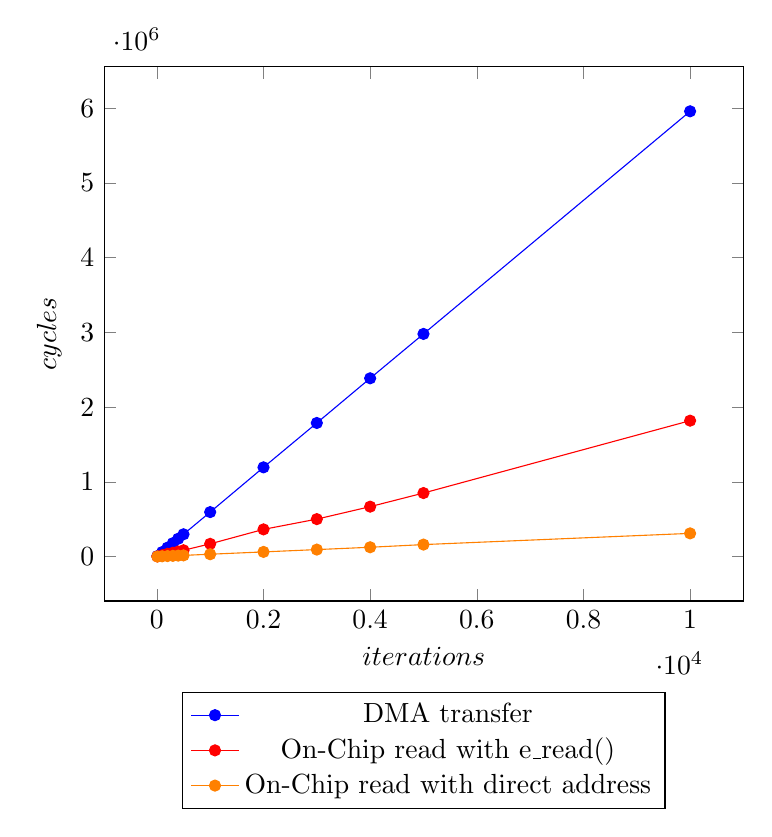
\begin{tikzpicture}
	\begin{axis}[
        xlabel=$iterations$,
        ylabel=$cycles$,
        legend style={at={(0.5,-0.17)},anchor=north},
        %xmode=log,
        %log basis x={10}
        width=0.8\textwidth
    ],
	\addplot[mark=*,blue] plot coordinates {
        (10,6000)
        (100,60000)
        (200,119242)
        (300,178631)
        (400,238313)
        (500,298039)
        (1000,595043)
        (2000,1194041)
        (3000,1788042)
        (4000,2386040)
        (5000,2980040)
        (10000,5960049)
    };
    \addlegendentry{\gls{DMA} transfer}
	\addplot[mark=*,red] plot coordinates {
        (10,1700)
        (100,17000)
        (200,36618)
        (300,50417)
        (400,67227)
        (500,84041)
        (1000,170000)
        (2000,363745)
        (3000,500980)
        (4000,667895)
        (5000,850000)
        (10000,1818769)
    };
    \addlegendentry{On-Chip read with e\_read()}
	\addplot[mark=*,orange] plot coordinates {
        (10,359)
        (100,3500)
        (200,6273)
        (300,9379)
        (400,12471)
        (500,15647)
        (1000,31000)
        (2000,62079)
        (3000,93061)
        (4000,124292)
        (5000,160000)
        (10000,310079)
    };
    \addlegendentry{On-Chip read with direct address}
	\end{axis}
\end{tikzpicture}
\caption{Performance measures based on number of cycles executed for a given number of iterations transferring 8 bits of data}
\label{graph transfert}
\end{figure}

\begin{figure}[h!]
\centering
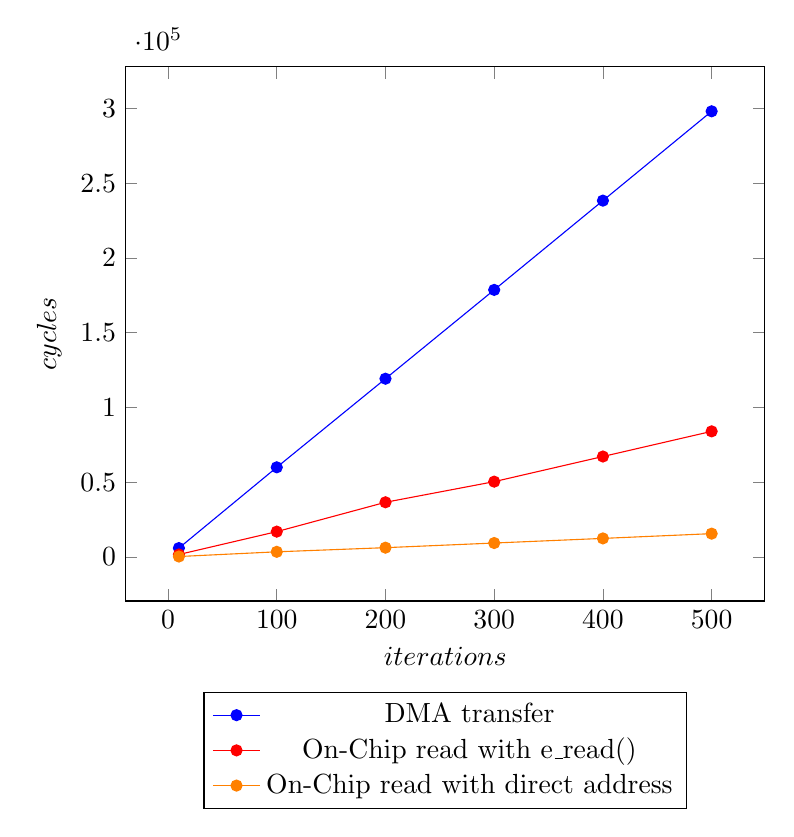
\begin{tikzpicture}
	\begin{axis}[
        xlabel=$iterations$,
        ylabel=$cycles$,
        legend style={at={(0.5,-0.17)},anchor=north},
        %xmode=log,
        %log basis x={10}
        width=0.8\textwidth
    ],
	\addplot[mark=*,blue] plot coordinates {
        (10,6000)
        (100,60000)
        (200,119242)
        (300,178631)
        (400,238313)
        (500,298039)
    };
    \addlegendentry{DMA transfer}
	\addplot[mark=*,red] plot coordinates {
        (10,1700)
        (100,17000)
        (200,36618)
        (300,50417)
        (400,67227)
        (500,84041)
    };
    \addlegendentry{On-Chip read with e\_read()}
	\addplot[mark=*,orange] plot coordinates {
        (10,359)
        (100,3500)
        (200,6273)
        (300,9379)
        (400,12471)
        (500,15647)
    };
    \addlegendentry{On-Chip read with direct address}
	\end{axis}
\end{tikzpicture}
\caption{Performance measures based on number of cycles executed for a given number of iterations transferring 8 bits of data, zoomed from 0 to 500 iterations}
\label{graph transfert2}
\end{figure}

It is important to note that we were only interested by measuring the transfer of a small amount of data. Using the \gls{DMA} is faster for bigger data size \cite{programmingadapteva}.


\section[Example 3]{Example: Transfer between host and eCores} \label{ex3}

Examples available on \href{https://github.com/nkcr/parallella-computing/tree/master/simple-epiphany/data-from-host-to-epiphany}{GitHub}\cite{githubproject}: \textit{simple-epiphany/data-from-host-to-epiphany}, \textit{simple-epiphany/data-from-host-to-eCore}.

The goal we want to reach is creating a shared space from the host, then filling it with data to be used by \glspl{eCore}.

Figure \ref{fig host to eCore} illustrates the process of how we will transfer data from the host to \glspl{eCore} (version a), or an individual \gls{eCore} (version b). We see that we can either use a shared memory buffer to set a memory available for every \glspl{eCore}, or we can directly write to an \gls{eCore}'s local memory. For the version \textit{a}, the steps are:

\begin{enumerate}
  \item[1a.] allocating the shared space (\code{e\_alloc}) from the host
  \item[2a.] filling the shared space (\code{e\_write}) from the host
  \item[3a.] loading \glspl{eCore} and make them use the shared space
\end{enumerate}

For the version \textit{b} the steps are simpler because we avoid the need of a shared memory buffer by directly writing to an \gls{eCore}'s local memory (\textit{1b}). Then, an \gls{eCore} can use it's local memory to read data set from the host (2b).

\begin{figure}[h!]
\centering
\includegraphics[width=0.7\textwidth]{examples/host_to_eCores.pdf}
\caption{Simplistic scheme of transferring data the host to \glspl{eCore}, or an individual \gls{eCore}}
\label{fig host to eCore}
\end{figure}

In this example, we will use 2 int arrays of 200 plus an array to store a result. Allocating memory and filling a shared buffer is not a tough task once we know how to use \code{e\_alloc} and \code{e\_write}. In the following code, we show the allocating and writing part:

\begin{lstlisting}
  e_mem_t shared_result;
  e_mem_t shared_x;
  e_mem_t shared_y;
  
  e_alloc(&shared_result, BUFOFFSET, ncores*sizeof(float));
  e_alloc(&shared_x, BUFOFFSET + ncores*sizeof(float), 
                                 200*sizeof(float));
  e_alloc(&shared_y, BUFOFFSET + ncores*sizeof(float) 
                               + 200*sizeof(float), 
                                 200*sizeof(float));
  
  float y[200];
  float x[200];
  for(i=0; i<200; i++) y[i] = x[i] = i;
  int status = e_write(&shared_x, 0, 0, 0x0, y, 
                       200*sizeof(float));
  printf("Status of shared_x writing: %i\n", status);
  status = e_write(&shared_y, 0, 0, 0x0, x, 
                   200*sizeof(float));
  printf("Status of shared_y writing: %i\n", status);
\end{lstlisting}

To get those buffers from the \gls{eCore}, one has just to set pointers to the right addresses. Getting the right addresses implies that we know exactly where memory is mapped. As seen in the first part of this document (section \ref{memory}), the linker description file (\gls{LDF}) gives us that information. In our case, shared memory starts at \code{0x8f00'0000}. Hence, we get our buffers starting with this base address plus an offset, corresponding each time to the cumulated size of the previous buffers. The following code shows the part on the \glspl{eCore}' source code where buffers are retrieved by setting pointers to corresponding addresses:

\begin{lstlisting}
  volatile float *result;
  volatile float *shared_x;
  volatile float *shared_y;
  
  result   = (volatile float *) (0x8f000000 + 0x4*num);
  shared_x = (volatile float *) (0x8f000000 + 16*sizeof(float));
  shared_y = (volatile float *) (0x8f000000 + 16*sizeof(float) 
                                            + 200*sizeof(float));
\end{lstlisting}

We can then use those buffers. In the following example, we read values from the x and y arrays then write a result to the result buffer. That result will tell us if the process successfully worked, because we will be able to read it from the host part:

\begin{lstlisting}
	*result = shared_matrix1[num] + shared_matrix2[num] 
	                              + num / 10.0;
\end{lstlisting}

Another way to write data from the host to the \gls{epiphany} is directly writing to an \gls{eCore}'s local memory. That method also uses the \code{e\_write} method. But, instead of giving as first parameter a shared\_buffer, we pass an \code{epiphany\_t} object, which represents a workgroup of \glspl{eCore} (see section \ref{workgroup}). We can then specify the \gls{eCore}'s coordinates, relative to the workgroup. 

The following code shows how a data is directly sent to an \gls{eCore}'s local memory:

\begin{lstlisting}
// Here we can select which eCore to unlock (eCore(0;1) there)
int ok = 1;
e_write(&dev, 0, 1, 0x4000, &ok, sizeof(int));
\end{lstlisting}

We note that we gave \code{0x4000} as the offset memory. That value corresponds to the relative offset memory of the local \gls{eCore}'s memory. As seen previously in this document, each \gls{eCore} has 4 banks of memory, starting from \code{0x0000} to \code{0x7fff}. Giving an offset of \code{0x4000} will write the data to the second bank of memory (see table \ref{table:eCore}).

From the \gls{eCore}, to read the values set from the host, we had to set a variable at the correct address. To make it easier, we declared a char array and specified it's location to be on the second bank of local memory (hence starting at the address \code{0x4000}). We then used that array to place or read the data. The following code shows how we declared the array and how we placed the data:

\begin{lstlisting}
	volatile int instructions[8] SECTION(".text_bank2"); // 0x4000
	// instruction[0] is at 0x4000
	// instruction[1] is at 0x4004
	int result = instructions[0]; // Data from the host
\end{lstlisting}


\section{Benchmark} \label{benchmark}

The point of this part is to implement the linpack benchmark test.Taking the existing c implementation, we will first simply run it only on the host part. We will then try to improve it by including the \gls{epiphany} in the process, using the \glspl{eCore}. We should be able to measure a better performance between the host only implementation and the one using the \gls{epiphany}.

The linpack works nearly out-of-the-box and only requires to adapt the \code{second} method, which is used to measure the performance. The result we obtained was approximately 120 MFlops, which is what we could expect from an ARM-A9 processor\cite{linpackpc}. We will now look at how we could include the \gls{epiphany} in the process.

Using linpack directly on the \gls{epiphany} won't work due to memory capacity (see figue \ref{code overflow}). What we will do is delegate jobs from the host to the \gls{epiphany}. To do so, we will set some data in the global memory, thus being available to the \glspl{eCore} and some status variables to know which \glspl{eCore} are already working or not. The host will have to poll each \glspl{eCore}' statuses, once it gets a free \gls{eCore} set to it some specific data required to compute and then tel the \gls{eCore} to do the work using global memory with it's specific data received from the host. Figure \ref{fig flow host} describes how the host part will interact. As long as there is still some work to do (more iterations), the host will look for a free \gls{eCore}, give to it some instructions and then release it.

\begin{figure}[h!]
\begin{lstlisting}[language=bash]
... ld: clinpack.elf section `.bss' will not fit in region `INTERNAL_RAM'
... ld: region `INTERNAL_RAM' overflowed by 318544 bytes
\end{lstlisting}
\caption{Memory capacity exceeded if using c linpack on the \gls{epiphany}}
\label{code overflow}
\end{figure}

\begin{figure}[h!]
\centering
\includegraphics[width=1\textwidth]{flow_linpack_host.png}
\caption{Activity diagram on the host side}
\label{fig flow host}
\end{figure}

On the \gls{epiphany} part (see figure \ref{fig flow epiphany}), each \gls{eCore} waits to be released by the host, compute what is needed using global data and specific ones (instructions), write the result and loops again. It is stopped only when application exits.

\begin{figure}[h!]
\centering
\includegraphics[width=1\textwidth]{flow_linpack_epiphany.png}
\caption{Activity diagram on the \gls{epiphany} side}
\label{fig flow epiphany}
\end{figure}

Using that process works for a small number of iterations. We implemented the concept inside a loop called once. But no relevant changes were observed since the section optimized did not represent a significant part of the benchmark. We had the same performance.

When profiling the linpack implementation (using \code{gprof}), we found out that approximately 88\% of the total running time spent by the benchmark is in one function (see figure \ref{code profilling}). That function (\code{daxpy}) makes the addition of an array plus an array multiplied by a constant. A more precise measure (using \code{gcov}), to see where the critical section is, showed us that the most used line within that function is called 69'679'500 times (see figure \ref{code profilling2}). So we will be focusing on optimizing this particular part of the code, which is the following code:

\begin{lstlisting}
for (i = 0;i < n; i++) {
  dy[i] = dy[i] + da*dx[i];
}
\end{lstlisting}

\begin{figure}[h!]
\begin{lstlisting}
Flat profile:

Each sample counts as 0.01 seconds.
  %   cumulative   self              self     total           
 time   seconds   seconds    calls  us/call  us/call  name    
 88.49      1.23     1.23  1060694     1.16     1.16  daxpy
  7.91      1.34     0.11                             matgen
  2.88      1.38     0.04                             dgefa
  0.72      1.39     0.01    20394     0.49     0.49  dscal
  0.00      1.39     0.00    20394     0.00     0.00  idamax
  
\end{lstlisting}
\caption{Results of the c linpack profilling using gprof}
\label{code profilling}
\end{figure}

\begin{figure}[h!]
\begin{lstlisting}
 69679500:  572:        for (i = 0;i < n; i++) {
 69679500:  573:                dy[i] = dy[i] + da*dx[i];
        -:  574:        }
\end{lstlisting}
\caption{c linpack Line profiling of the most used line using gcov}
\label{code profilling2}
\end{figure}

Using the process we described previously (fig \ref{fig flow host} and fig \ref{fig flow epiphany}), we faced a critical deadlock while executing the program. After a while, all \glspl{eCore} were in a busy state and didn't change their state ever. 

Trying to solve the problem, we saw that it never happened after the same number of iterations. To get a better idea of what could cause the deadlock, we made a merged activity diagram showing data access (figure \ref{fig flow general}). It seemed that status variable was read both at the same time by the \gls{epiphany} and the host side, it could have been the source of our deadlock.

\begin{figure}[h!]
\centering
\noindent\makebox[\textwidth]{\includegraphics[width=1.4\textwidth]{flow_general.pdf}}
\caption{General activity diagram}
\label{fig flow general}
\end{figure}

From figure \ref{fig flow general}, we developed another activity diagram preventing the program accessing the same variable at the same time (figure \ref{fig flow general V2}). That way, we would use shared memory and local \glspl{eCore}' memory. It would prevent the host and \gls{epiphany} side polling the same variables at the same time.

\begin{figure}[h!]
\centering
\noindent\makebox[\textwidth]{\includegraphics[width=1.4\textwidth]{flow_general_V2.pdf}}
\caption{General activity diagram second version using \glspl{eCore}' local memory}
\label{fig flow general V2}
\end{figure}

\subsection{When hardware meets software}

Before implementing our second activity diagram (fig \ref{fig flow general V2}) and after some time testing some possibilities of what could cause our deadlock, we observed a curious fact: our program always took more time to come to a deadlock when it was used after a time of inactivity. It is shown in graph \ref{graph deadlock temp}. Based on this observation, we suspected temperature to be involved in our problem. After more precise measures, it came that temperature was definitely the cause of our deadlock. As shown in graph \ref{graph deadlock temp2}, above 69°C, system became instable and gave unpredictable results. Looking at adapteva's hardware github repos \cite{githubadaptevahard}, we found out that an issue warns us about the parallella becoming unstable under unless cooled properly\cite{githubadaptevahardissue}. This new factor will then be watched in our future implementation. Graph \ref{graph deadlock temp} and \ref{graph deadlock temp2} show number of iterations and temperature after and before a launch of our program. We measured temperature of the parallella, then we launched our program and measured temperature reached when deadlock occurred as well as number of iterations executed. It is not surprising to observe that if the parallella is cooler, number of iteration before deadlock increases accordingly (graph \ref{graph deadlock temp}). Deadlocks in our measures start from 69.2°C to 70.6°C (graph \ref{graph deadlock temp2}. Measuring a pertinent range of temperature was a tough task because, after each test, the parallella was at it's warmest. We had to cool the heatsink, wait, or use a fan. In some cases, the parallella could have been harder to warm because we would have cooled the heatsink, thus taking more time and giving more iterations before coming to a deadlock.

Leaving from this observation, we will now be more careful to properly cool the parallella by adding a fan or placing it in a cooler area. We leave the final implementation of the linpack for the next chapter.

%\begin{tikzpicture}
%\begin{axis}[
%	title={Grids with shader=faceted interp}]
%
%\addplot3[patch,patch refines=3,
%		shader=faceted interp,
%		patch type=biquadratic]
%coordinates {
%	%(47.7,69.2,108788)
%	(66.1,69.6,1603)
%	(66.6,69.6,2902)
%	(66.6,70.6,1021)
%	(66.8,69.8,860)
%	(67.4,69.8,1399)
%	(66.9,69.5,364)
%	(66.9,70.1,1260)
%	(67.6,70.2,609)
%	(67.4,69.8,181)
%	
%	%(52.1,69.6,89814)
%	(66.0,69.6,2101)
%	(66.9,69.8,3291)
%	(67,70.6,1865)
%	(67.5,70,953)
%	(66.6,70.1,854)
%	(67.4,69.8,847)
%	(67.6,70,1025)
%	(67.4,69.7,164)
%	(67.5,69.8,1058)
%	
%	%(51.5,69.3,90775)
%	(65.8,69.8,2798)
%	(66.6,69.8,1699)
%	(66.3,69.6,645)
%	(67.3,70,804)
%	(66.9,70.2,1496)
%	(67.4,70.1,793)
%	(66.9,70.2,678)
%	(67.3,70.1,942)
%	(66.9,69.6,882)
%};
%\end{axis}
%\end{tikzpicture}

\begin{figure}
\centering
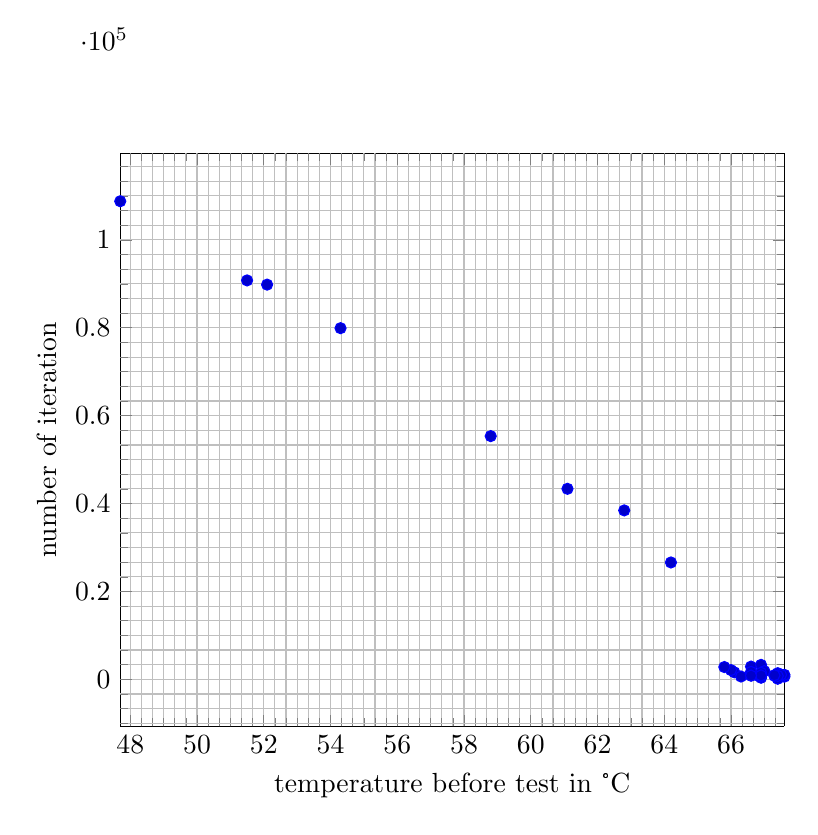
\begin{tikzpicture}
\begin{axis}[view={0}{0},
	grid=both,
	minor tick num=5,
	scale only axis,
	only marks,
	xlabel=temperature before test in °C,
	ylabel=temperature when blocked in °C,
	zlabel=number of iteration]
\addplot3+[] 
coordinates {
	(47.7,69.2,108788)
	(66.1,69.6,1603)
	(66.6,69.6,2902)
	(66.6,70.6,1021)
	(66.8,69.8,860)
	(67.4,69.8,1399)
	(66.9,69.5,364)
	(66.9,70.1,1260)
	(67.6,70.2,609)
	(67.4,69.8,181) % e
	(52.1,69.6,89814)
	(66.0,69.6,2101)
	(66.9,69.8,3291)
	(67,70.6,1865)
	(67.5,70,953)
	(66.6,70.1,854)
	(67.4,69.8,847)
	(67.6,70,1025)
	(67.4,69.7,164)
	(67.5,69.8,1058) % e
	(51.5,69.3,90775)
	(65.8,69.8,2798)
	(66.6,69.8,1699)
	(66.3,69.6,645)
	(67.3,70,804)
	(66.9,70.2,1496)
	(67.4,70.1,793)
	(66.9,70.2,678)
	(67.3,70.1,942)
	(66.9,69.6,882) % e
	(61.1,69.3,43354)
	(58.8,69.3,55343)
	(54.3,70.2,79905)
	(64.2,70,26593)
	(62.8,70.3,38439) % repeat
	(66.6,70.1,854)
};

\end{axis}
\end{tikzpicture}
\caption{Temperature before test vs the number of iterations reached just before deadlock}
\label{graph deadlock temp}
\end{figure}

\begin{figure}
\centering
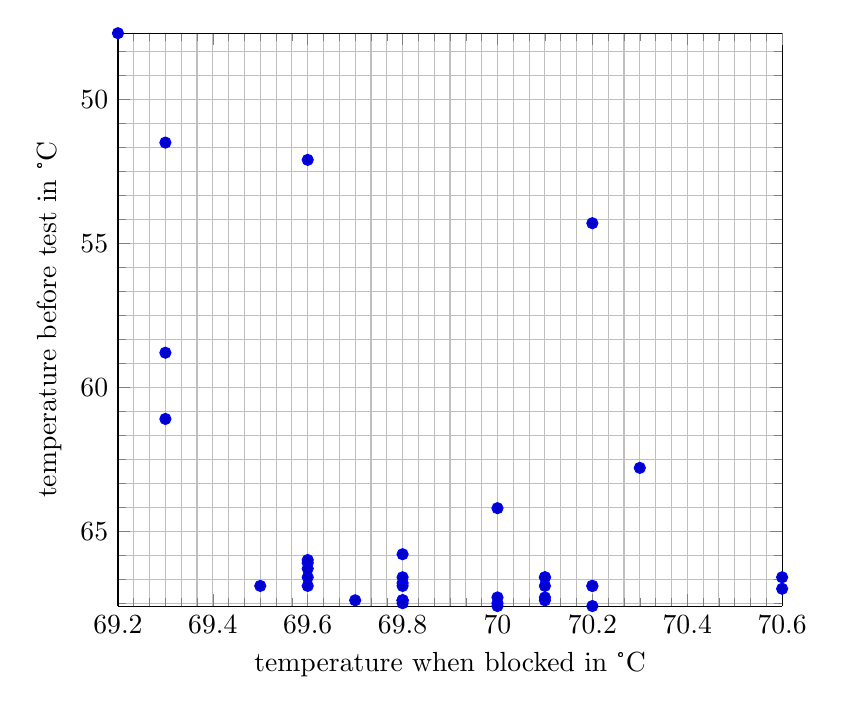
\begin{tikzpicture}
\begin{axis}[view={90}{90},
	grid=both,
	minor tick num=5,
	scale only axis,
	only marks,
	xlabel style={rotate=90},
	xlabel=temperature before test in °C,
	ylabel=temperature when blocked in °C,
	zlabel=number of iteration]
\addplot3+[] 
coordinates {
	(47.7,69.2,108788)
	(66.1,69.6,1603)
	(66.6,69.6,2902)
	(66.6,70.6,1021)
	(66.8,69.8,860)
	(67.4,69.8,1399)
	(66.9,69.5,364)
	(66.9,70.1,1260)
	(67.6,70.2,609)
	(67.4,69.8,181) % e
	(52.1,69.6,89814)
	(66.0,69.6,2101)
	(66.9,69.8,3291)
	(67,70.6,1865)
	(67.5,70,953)
	(66.6,70.1,854)
	(67.4,69.8,847)
	(67.6,70,1025)
	(67.4,69.7,164)
	(67.5,69.8,1058) % e
	(51.5,69.3,90775)
	(65.8,69.8,2798)
	(66.6,69.8,1699)
	(66.3,69.6,645)
	(67.3,70,804)
	(66.9,70.2,1496)
	(67.4,70.1,793)
	(66.9,70.2,678)
	(67.3,70.1,942)
	(66.9,69.6,882) % e
	(61.1,69.3,43354)
	(58.8,69.3,55343)
	(54.3,70.2,79905)
	(64.2,70,26593)
	(62.8,70.3,38439) % repeat
	(66.6,70.1,854)
};

\end{axis}
\end{tikzpicture}
\caption{Temperature reached when deadlock occurred along with temperature when started}
\label{graph deadlock temp2}
\end{figure}

%\begin{tikzpicture}
%\begin{axis}[
%    ybar,
%    enlargelimits=0.15,
%    legend style={at={(0.5,-0.15)},
%      anchor=north,legend columns=-1},
%    ylabel={\#participants},
%    symbolic x coords={m1,m2,m3},
%    xtick=data,
%    nodes near coords,
%    nodes near coords align={vertical},
%    ]
%\addplot coordinates {(m1,47.7)   (m2,66.1) (m3,66.6)  };
%\addplot coordinates {(m1,69.2)   (m2,69.6) (m3,69.6) };
%\addplot coordinates {(m1,108788) (m2,1603) (m3,2902) };
%\legend{used,understood,not understood}
%\end{axis}
%\end{tikzpicture}

\section{Conclusion}

We learnt in this chapter how to transfer data among the host and the \glspl{eCore}. If we understand well how memory is mapped and how the \glspl{SDK} provided by Adapteva work, it is not a tough task. Knowing how data transfers work is essential to start developing on the parallella, it will allow us to properly make \glspl{eCore} communicating among them and with the host. We also reached the physical limits of the parallella, either by trying to fit the linpack implementation on the \gls{epiphany}, reaching its memory limit, or by under cooling the parallella until it became instable. What we learnt from those examples and observations will be useful for the next chapter. Let's move to some practical examples.